\documentclass[thesis.tex]{subfiles}

\begin{document}

    \section{Analysis of wafer 292}
    \label{sec:wafer292}

        Of wafer 292, the membranes 292c and 292d have been measured. The pores were opened by floating as explained in \cref{sssec:barrier-layer-dissolution}. The thickness of the membranes is
        \begin{equation}
            l_\mathrm{pore}=\SI{60}{\micro\meter}.
        \end{equation}
        Expected is an absorption and desorption isotherm with a hysteresis as explained in \cref{sssec:open-funnelled-pores}.
        While by theory, the condensation branch is supposed to be steeper than the evaporation branch, the measurements show the opposite.
        The condensation seems to have a tail to lower pressures. This can be explained by inhomogenuous pore openings. In fact, the membrane's
        pores were not well opened after the first barrier layer dissolution process (compare \cref{sssec:barrier-layer-dissolution}), as determined
        from MEB views, and has therefore been opened using a second floating process. That might have cause an increase of the funneling and/ or
        corrugations and also left some bad open pores.


    \section{Analysis of wafer 296}
    \label{sec:wafer296}

      As already mentioned in \cref{sssec:barrier-layer-dissolution}, the \textit{barrier layer} dissolution shall be taken a closer look at. The reason for this is explained in the following. Therefore, some analysis of wafer 295, which has not yet been introduced, needs to be done at this place. The more detailed analysis of wafer 295 will be done in \cref{sec:wafer295}, though.
      \medskip

      Following, the pore opening of membrane 295 c shall be inspected:

      After $t_1^{295c}$ of floating on phosphoric acid, white speckles appear on the wafer. As this phenomenon looks similar to the observation made during the absorption process of an isotherm, this can be interpreted as the membrane filling with the acid. Due to the capillary flow rate of phosphoric acid in pores of diameter $d_\mathrm{pore}^{295c}=\SI{40}{\nano\meter}$, a single pore fills within $t_\mathrm{fill}^{295}=\SI{5}{\second}$ ??? quote physical basics ???. That the milky aspects occur over about $\Delta t^{295c} = \SI{3}{\minute}$ implies that some pores fill minutes before others. Therefore, the pore size distribution is increased during this time. The caused distribution in radius can be approximated by the etch rate of the acid.

      The barrier layer's thickness of wafer 295 is about $d_\mathrm{barrierlayer}^{295c}=\SI{30}{\nano\meter} $ as observed on the MEB views shown in \cref{fig:295c_barrier_layer}. As the first milky speckles appear after $t_1^{295c}=\SI{20}{\minute} $, the etch rate is about
      \begin{equation}
          e = \SI{1,5}{\nano\meter\per\minute}. \label{eq:etch-rate}
      \end{equation}
      This yields a diameter distribution of
      \begin{equation}
          \Delta d_1^{295c} = \SI{9}{\nano\meter}
      \end{equation}
      which is only due to the opening process of the pores. Furthermore, the wafers are left floating until the whole upper side is observably covered by a liquid film (compare figure???). This state has been reached after $t_\mathrm{2}^{295c}=\SI{40}{\minute} $ of floating. Thus, by the theory explained above, the pores should widen by up to
      \begin{equation}
          \Delta d_2^{295c} =\SI{60}{\nano\meter}.
      \end{equation}
      \medskip

      \begin{figure}
        \subfloat[]{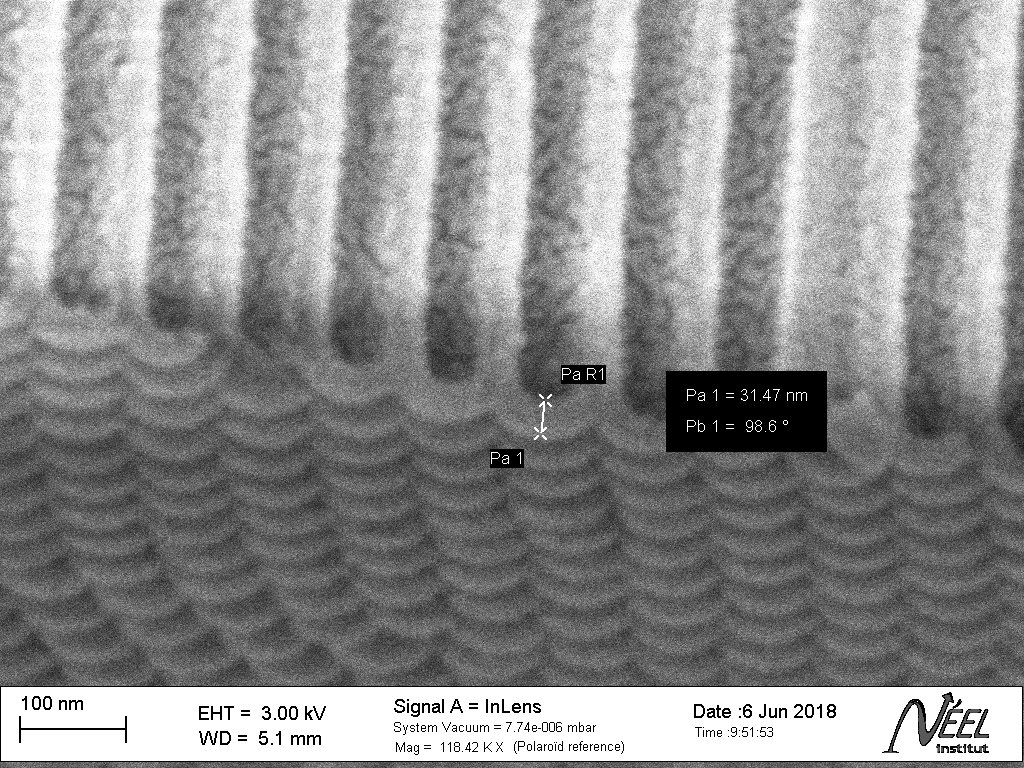
\includegraphics[width=0.45\textwidth]{images/295c_barrier_layer.jpg}
          \label{fig:295c_barrier_layer}}
        \hfill
        \subfloat[]{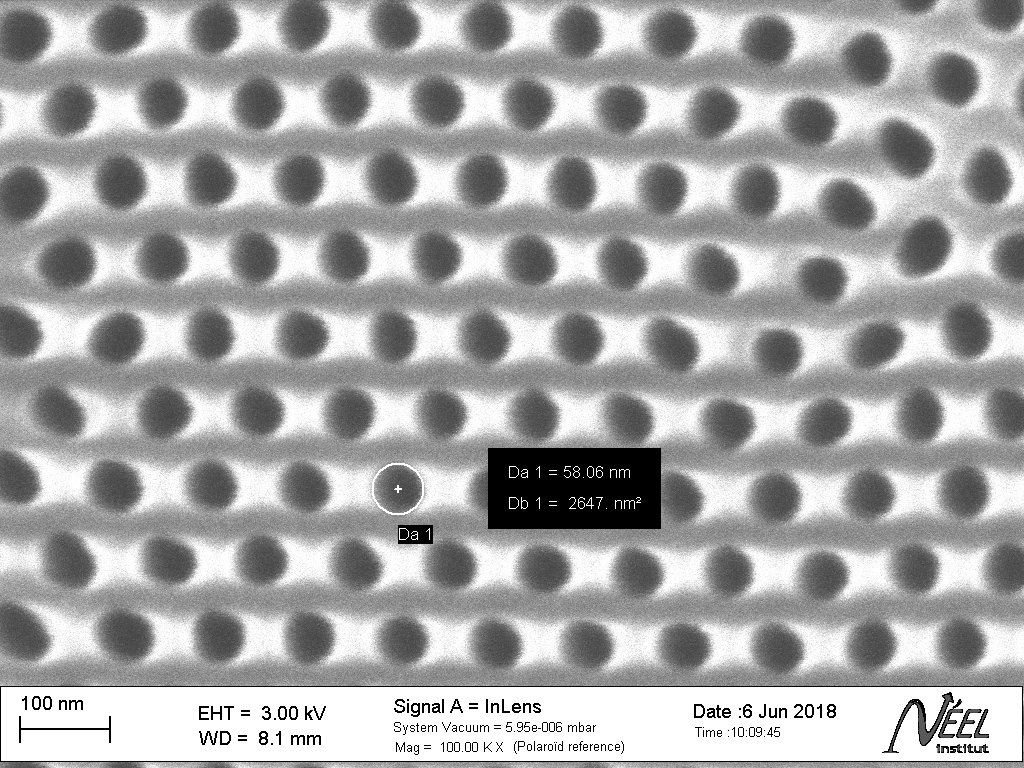
\includegraphics[width=0.45\textwidth]{images/295c_pores.jpg}
          \label{fig:295c_pores}}
        \caption{MEB views of membrane 295c. The thickness of the \textit{barrier layer} is measured directly with the \textsc{Zeiss} software in \protect\subref{fig:295c_barrier_layer}. As the membrane is not oriented exactly orthogonal to the microscope and the perspective of the layer is a bit distortet, the value can only be used as a rough approximation. \protect\subref{fig:295c_pores} shows the pores on the solution side of the membrane.}
      \end{figure}

      Summing up the section above, the pore diameters should be distributed around
      \begin{equation}
          d_\mathrm{pore}^\mathrm{295c-theory} = \SI{109}{\nano\meter}.
      \end{equation}
      The analysis of the MEB vues of the membrane yield a diameter distribution around
      \begin{equation}
          d_\mathrm{pore}^\mathrm{295c-MEB} = \SI{58}{\nano\meter},
      \end{equation}
      though. Thus, at some point there must be a mistake in the interpretation of the observations.
      \medskip

      The idea behind the following experiments with waver 296 is to better understand what happens during the \textit{barrier layer} dissolution process and to find a systematic way to open the pores with a minimal pore diameter increment and diameter distribution increment. Floating and immersing single membranes in phosphoric acid shall lead to a calibration of the respecting etch rates $e_\mathrm{float}$ and $e_\mathrm{immerse}$.
      \medskip

      The thickness of wafer 296 is
      \begin{equation}
          l^{296}_\mathrm{pore}=\SI{60}{\micro\meter}.
      \end{equation}
      As explained before in \cref{sssec:barrier-layer-dissolution}, this wafer shall be used to further understand the barrier layer dissolution. The goal is to be able to produce the membranes in a more controlled way an to hereby reduce the funneling aspect of the pores. \cref{fig:wafer-296} shows the treatments of the membranes and gives an overview over the conducted measurements. While the membranes 296c and 296d are immersed in phosphoric acid for
      \begin{align}
          \begin{split}
              t^\mathrm{296c}_\mathrm{immerse}=\SI{6,5}{\minute},    \\
              t^\mathrm{296d}_\mathrm{immerse}=\SI{13}{\minute},
          \end{split}
          \label{eq:t-immerse}
      \end{align}
      296e and 296f are only floated on the acid on the barrier layer side for
      \begin{align}
          \begin{split}
              t^\mathrm{296e}_\mathrm{float}=\SI{13}{\minute}, \\
              t^\mathrm{296f}_\mathrm{float}=\SI{26}{\minute}
          \end{split}
          \label{eq:t-float}
      \end{align}
      respectively. Assuming the etch rate to be equal for both sides of the barrier layer, meaning from within the pore and from the outside, the thickness of the barrier layer of 296c and 296e and also of 296d and 296f should be equal after the dissolution. Moreover, all pores should still be closed assuming an etch rate of approximately $\SI{1}{\nano\meter\per\minute}$. The latter should be clearly visible on the volumetric measurements. Furthermore, only the pores of the immersed membranes are expected to be widened. The horizontal etch rate, which according to \cref{sssec:barrier-layer-dissolution} must be different from the one attacking the barrier layer vertically, shall be put a figure to in the run of the evaluations.

      \subfile{tikz/wafers/wafer_296_processing_plan.tex}

      \Cref{fig:full-comp-w296} shows a full comparison of the volumetric measurements of the membranes mentioned above. Additionally, membrane 296a (closed pores) and 296b before and after the barrier layer dissolution are presented on the graph. So the membranes 296a and 296b cp serve as reference for closed pore membranes, while 296b op serves for open pore membranes. The comparison of the different membranes implies that indeed, all pores are still closed for the four treated membranes as the shapes of their isotherms match the one of 295a and 296b cp while they do not match the one of 296b op. Moreover, no big diameter variation can be observed. Which cannot be observed though, that is weather the pores already have microscopic openings on the barrier layer side. If that were the case, hexane would condense there at spinodal pressures lower than the equilibrium pressure of the small ends. Hereby, the pores would be left in a closed shape. This case would not be visible on the volumetric measurements as the condensed amount of hexane necessary to close the pores were so small. If the openings were so large already as for the spinodal pressure to be larger than the equilibrium pressure of the small end, that case would be visible on the isotherm because whole pores would fill at higher pressures. Therefore, the latter case can be excluded.

      Next, the floated and immersed membranes shall be regarded separately.

      \subfile{tikz/graphs/296_membranes/296_membranes.tex}


      \subsection{Floated membranes 296e and 296f}
      \label{subsec:floated-membranes}

          The comparison of the volumetric measurements of the membranes 296e, 296f and for the reference of an untreated membrane 296a are shown in \cref{fig:full-comp-w296}. Even though the wafer has been produced as a whole and the membranes 296e and 296f have only been floated on ??? acid without opening the pores, by theory leaving the pore diameters unchanged, a clear offset in diameter between 296a and the other two membranes is visible. As 296e and 296f are pretty superimposed though and also the shapes of isotherms match according to \cref{sec:wafer296}, no error in the before made interpretations of the pores still being closed can be implied. This leaves only the possibility of the pore diameters being distributed throughout the wafer and hereby throughout the membranes.

          As a reminder, all the pores are closed. Regarding the light transmission measurement, the transmission dips of condensation and evaporation are expected to be of the same magnitude as both proccesses occur at equilibrium pressure. Unlike theory, \cref{fig:full-comp-w296} shows deeper transmission minima for the condensation than it does for the evaporation. This cannot be explained by the theory explained in \cref{subsec:light-transmission-interpretation}. One possible approach could be the corrugations within the single pores that lead to an unreversible absorption and desorption isotherm.

          \subfile{tikz/graphs/296_a_e_f/296_a_e_f.tex}


      \subsection{Immersed membranes 296c and 296d}
      \label{subsec:immersed-membranes}

          \subfile{tikz/graphs/immersion_experiment/immersion.tex}

          \Cref{fig:immersed-comp-w296} compares the volumetric and also the transmission measurements of the immersed membranes 296c and 296d, again adding the untreated membrane 296a. As explained in \cref{sssec:cfp-leo}, condensation and evaporation in a closed funnelled pore occur at equilibrium pressure. Pores that are open on the large end start filling from the bottom and evaporating from the top so, regarding the isotherms in \cref{fig:immersed-comp-w296}, the lower end of the isotherm rising represents the small bottom end of the pores. This lower end of all three isotherms seems to be superimposed while the top end, representing the large open end of the pores, moves to larger diameters for longer immersion times. As the effect seems to occur linearly over the whole length of the pores, the acid seems to be saturating within the pores losing etching power. By \cref{sssec:cfp-leo}, the process can be visually interpreted as a pore straightening as shown in \cref{fig:funneling_increase}. Moreover, the increase of the funnelling aspect seems to be linear at least within the first 13 minutes of the immersion as doubling the immersion time yields double the diameter shift on the volumetric isotherm (compare \cref{eq:t-immerse}).

          \subfile{tikz/wafer_analysis/funnelling_increase.tex}


    \section{Analysis of wafer 295}
    \label{sec:wafer295}

        Wafer 295 is only
        \begin{equation}
            l^{295}_\mathrm{pore}=\SI{30}{\micro\meter}
        \end{equation}
        thick. Hereby, the effect of the funneling observed upon the previously measured membranes of a thickness of
        \begin{equation}
            l^{292,293,294,296}_\mathrm{pore}=\SI{60}{\micro\meter}
        \end{equation}
        is expected to be reduced. Assuming that the funneling aspect is linear implies a reduction of the effect by half.
        Finally, the membranes' pore diameters are reduced using ALD. \Cref{fig:wafer_295} shows the treatments and measurements of the inspected membranes of wafer 295.

        \subfile{tikz/wafers/wafer_295_processing_plan.tex}

        \subsection{Membrane 295a}

            \subfile{tikz/graphs/295a/295a.tex}

            To start with, membrane 295a shall be analysed. It is untreated, meaning that the pores are still closed on one end by the barrier layer. Expected are straight pores of a diameter of approximately
            $\SI{40}{\nano\meter}$ diameter with a significantly reduced funneling aspect resulting in a rather upright evaporation isotherm. The result is displayed in \cref{fig:295a}. The absorption and desorption isotherm shows a kink at two thirds of the height, which cannot easily be explained. While for straight pores, a straight isotherm rising is expected, the observed kink could speak for a deformation as shown in \cref{fig:weird_funnelling}, assuming that it is due to intra pore defects, not inter pore defects. Regarding inter pore defects, a discreet pore diameter variation could cause this shape of isotherm. Again, the reason for such a discreet distribution in pore sizes is not clear.

            \subfile{tikz/wafer_analysis/weird_pore_funnelling.tex}


            \subsubsection{Membrane 295a - after aluminum dissolution bath}

                Membrane 295a is measured again after a bath in the acid used for the aluminum dissolution as explained in \cref{sssec:al-dissolution}. The point of this is to see, if the  wafers immersion in the acid when dissolution the remaining aluminum after the anodizing might cause any unexpected defects or pore widening already. As the anodizing of wafer 295 has been conducted with the same parameters as the other wafers before (for instance wafer 296, the pore diameters are expected to be approximately the same. Referring to wafer 296 the pore diameters of
                \begin{equation*}
                    d_\mathrm{pore}^\mathrm{296a} = \SI{45\pm 5}{\nano\meter}
                \end{equation*}
                do not fit the ones results of membrane 295a with???
                \begin{equation*}
                    d_\mathrm{pore}^\mathrm{295a} = \SI{55\pm 6}{\nano \meter}.
                \end{equation*}
                Finally, the probing of the aluminum dissolution process, which by theory is not supposed to attack the alumina of the membranes and therefore has not been taken a deeper look at, yields the before and after result displayed in \cref{fig:295a_al_diss}. In between the two measurements, the membrane has been immersed for
                \begin{equation*}
                    t_\mathrm{immerse} = \SI{4,5}{\hour}
                \end{equation*}
                in ??? acid at a temperature of
                \begin{equation*}
                    T_\mathrm{acid} = \SI{0}{\celsius}.
                \end{equation*}
                The aluminum dissolution of the wafers takes approximately
                \begin{equation}
                    t_\mathrm{Al diss.} = \SI{4}{\hour}
                \end{equation}
                and uses the same parameters which makes for a relevant approximation of what changes to the pores are expected during the before mentioned production step. The change to the pore diameters is
                \begin{equation}
                    \Delta d_\mathrm{pore}^\mathrm{Al diss.} = \SI{3}{\nano\meter}.
                \end{equation}
                Both, the starting points of the condensation rise and of the evaporation drop are shifted in the same way. Moreover, the hysteresis did not increase during the process. These two observations speak for the pore widening being homogeneous and also the corrugations not having increased during the etching. Therefore, the production step of the aluminum dissolution conducted as explained in \cref{sssec:al-dissolution} can be disregarded as a cause of big pore impurities.

                \subfile{tikz/graphs/295a_before_after_al_diss_bath/295a_before_after.tex}


        \subsection{Membrane 295d, 295e, 295f, 295g}

            The membranes 295d, 295e, 295f, 295g yield very upright isotherms without any kinks or transmission defects. On the contrary, the membranes 295e and 295f superimpose perfectly, while 295d and 295g are only shifted to larger diameters ???. For all the membranes, the transmission dips of absorption and desorption show the same value. This can only be explained by almost perfectly straight pores if the disorder theory in \cref{subsec:light-transmission-interpretation} are assumed to be correct. Also, regarding the conversion to pore diameters according to \textsc{Kelvin} equation (compare \cref{sec:kelvin-equation}, the funneling aspect is the weakest so far measured in this experiment. This can be explained by the inverse of the effect observed upon the opening experiments of wafer 296 ???.

            \subsubsection{Membrane 295g}

              Finally, membrane 295g shall be assumed to be good enough in the sense of pore size distributions, funnelling and corrugations as to be used to check on the theories of condensation and evaporation in confinement. From the untreated MEB images, the difference of pore sizes on the aluminum and solution side, which are due to the funnelling aspect of the pores, can be approximated. To this end, the values
              \begin{equation}
                \begin{split}
                  d_\mathrm{pore}^\mathrm{Sol}=\SI{67}{\nano\meter}  \\
                  d_\mathrm{pore}^\mathrm{Al}=\SI{60}{\nano\meter}.
                \end{split}
                \label{eq:295g_pore_sizes}
              \end{equation}
              Moreover, the funnelling is assumed to be linear in the following. Therefore, the threshhold, that needs to be set for the distribution analysis for solution and aluminum side respectively, can be adapted using some basic geometry:
              \medskip

              \begin{figure}[htp]
                \centering
                \subfloat[]{%\includegraphics{images/AAM_295_PO_g_Al_06.tif}
                \label{fig:MEB_295g_al_side}}
                \hfill
                \subfloat[]{%\includegraphics{images/AAM_295_PO_g_Al_06.tif}
                \label{fig:MEB_295g_sol_side}}
                \caption{MEB images of membrane 295g of aluminum \protect\subref{fig:MEB_295g_al_side} and solution side \protect\subref{fig:MEB_295g_al_side}. The measurements of the pore diameters were done immediately using the \textsc{Zeiss} software of the microscope.}
                \label{fig:MEB_295g}
              \end{figure}





        \subsection{Membrane 295c}



\end{document}
